\section{Architektur}
\label{sec:arch}

Zu Anfang ist es sinnvoll, die Architektur des Systems festzulegen.
Diese bestimmt, welche Komponenten und Microservices entwickelt und verbunden werden müssen.
Der erste Schritt dabei ist es, die Aufgaben aufzuteilen, die das System erfüllen soll.
Diese Aufgaben werden dann auf Microservices verteilt.
Die weitere Entwicklung des Systems stützt sich dann auf die fertige Architektur.

\subsection{Aufgabenverteilung}
Durch die Verwendung von \textit{Apache Spark} ist es nicht sinnvoll, dass Laden der Daten, die Deltaerkennung und das Speichern zu trennen.
In \textit{Apache Spark} werden alle drei Arbeitsschritte auf einem DataFrame ausgeführt.
Das heißt, dass dieses zwischen den Microservices ausgetauscht werden müsste, was zu einem erheblichen Aufwand führen würde.
Aus diesem Grund kann die logische Aufteilung in Ingestion, Deltaerkennung und Speicherung nicht auch als Aufgabenverteilung verwendet werden.

Besser trennbare Aufgaben findet man bei der Betrachtung der technischen Seite.
Hierbei gibt es die API, die Ingestion in \textit{Apache Spark} und das kontinuierliche Ausführen.

Bei der \textbf{API} handelt es sich um den Service für die Interaktion mit dem Data-Lake-System.
Durch die Anforderungen ist bereits festgelegt, dass dieser ein Web-Server mit einer REST-Schnittstelle ist.
Es geht zwar in dieser Arbeit nur um die Ingestion, aber der API-Service sollte Schnittstellen zu allen Funktionen des Data-Lake-Systems enthalten.

Die \textbf{Ingestion} ist dafür zuständig, die Datenquellen zu verarbeiten und den kompletten Prozess vom Laden bis zum Speichern der Daten in \textit{Apache Spark} auszuführen.
Die Ausführung soll für eine Datenquelle nur einmal gleichzeitig aber parallel für unterschiedliche laufen.

Bei einer zeitgesteuerten oder Datenstrom-Ingestion muss die \textbf{kontinuierliche Ausführung} sichergestellt werden.
Für alle Datenquellen muss regelmäßig geprüft werden, ob für diese gerade eine Ingestion ausgeführt wird und ausgeführt werden sollten.
Falls keine ausgeführt wird aber sollte, wird die Ingestion für diese Datenquelle gestartet.

\subsection{Komponenten und Microservices}
Die drei oben genannten Aufgaben können jeweils einem Microservice zugeordnet werden.
In \fref{fig:ingestion_arch} ist eine dazu passende Architektur zu sehen.
Der API-Service übernimmt die REST-Schnittstelle, der Ingestion-Service kümmert sich um die Ausführung der Ingestion und der Continuation-Service stellt die kontinuierliche Ausführung sicher.

Neben diesen Mircoservices wird noch ein Nachrichtensystem benötigt.
Das Nachrichtensystem stellt die Kommunikation zwischen den Microservices dar.
Hier ist es wichtig, dass es einem Sender möglich ist, Nachrichten an einen oder auch an mehrere Empfänger zu senden.
So soll sichergestellt werden, dass bestehende Microservices einfach repliziert und neue eingefügt werden können.

Zum Ablegen von internen Informationen wird eine Datenbank benötigt.
Alle Microservices haben zugriff auf diese Datenbank und können Daten in ihr bearbeiten.
Es handelt sich dabei aber nicht um den internen Speicher für geladene Daten des Data-Lake-Systems sondern nur um Daten, die für den Betrieb des Systems benötigt werden.
Darunter fallen zum Beispiel Authentifizierungsdaten oder Verbindungsinformationen von Datenquellen.

\begin{figure}
  \centering
  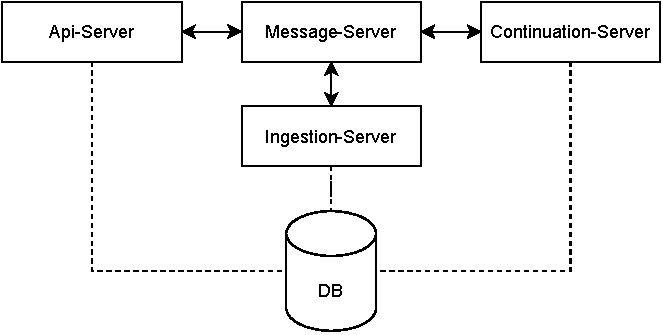
\includegraphics{Grafiken/ingestion-arch.pdf}
  \caption{Architektur der Ingestion Komponenten}
  \label{fig:ingestion_arch}
\end{figure}
